\documentclass{gescons}

\genre {Parceria}
\author{Ricardo Rezende}
\authorrole{Voluntário do Setor Comercial da Editares}
\title{Editares e IIPC Retomam Parceria para Ampliar a Venda de Livros}

\begin{document}
    \makeentrevistatitle
    %\maketitle

    %\fullwidthimage{fields}{b}

    \coverart{articles/parceria/fundo-parceria.png}
    
    

\begin{center}
    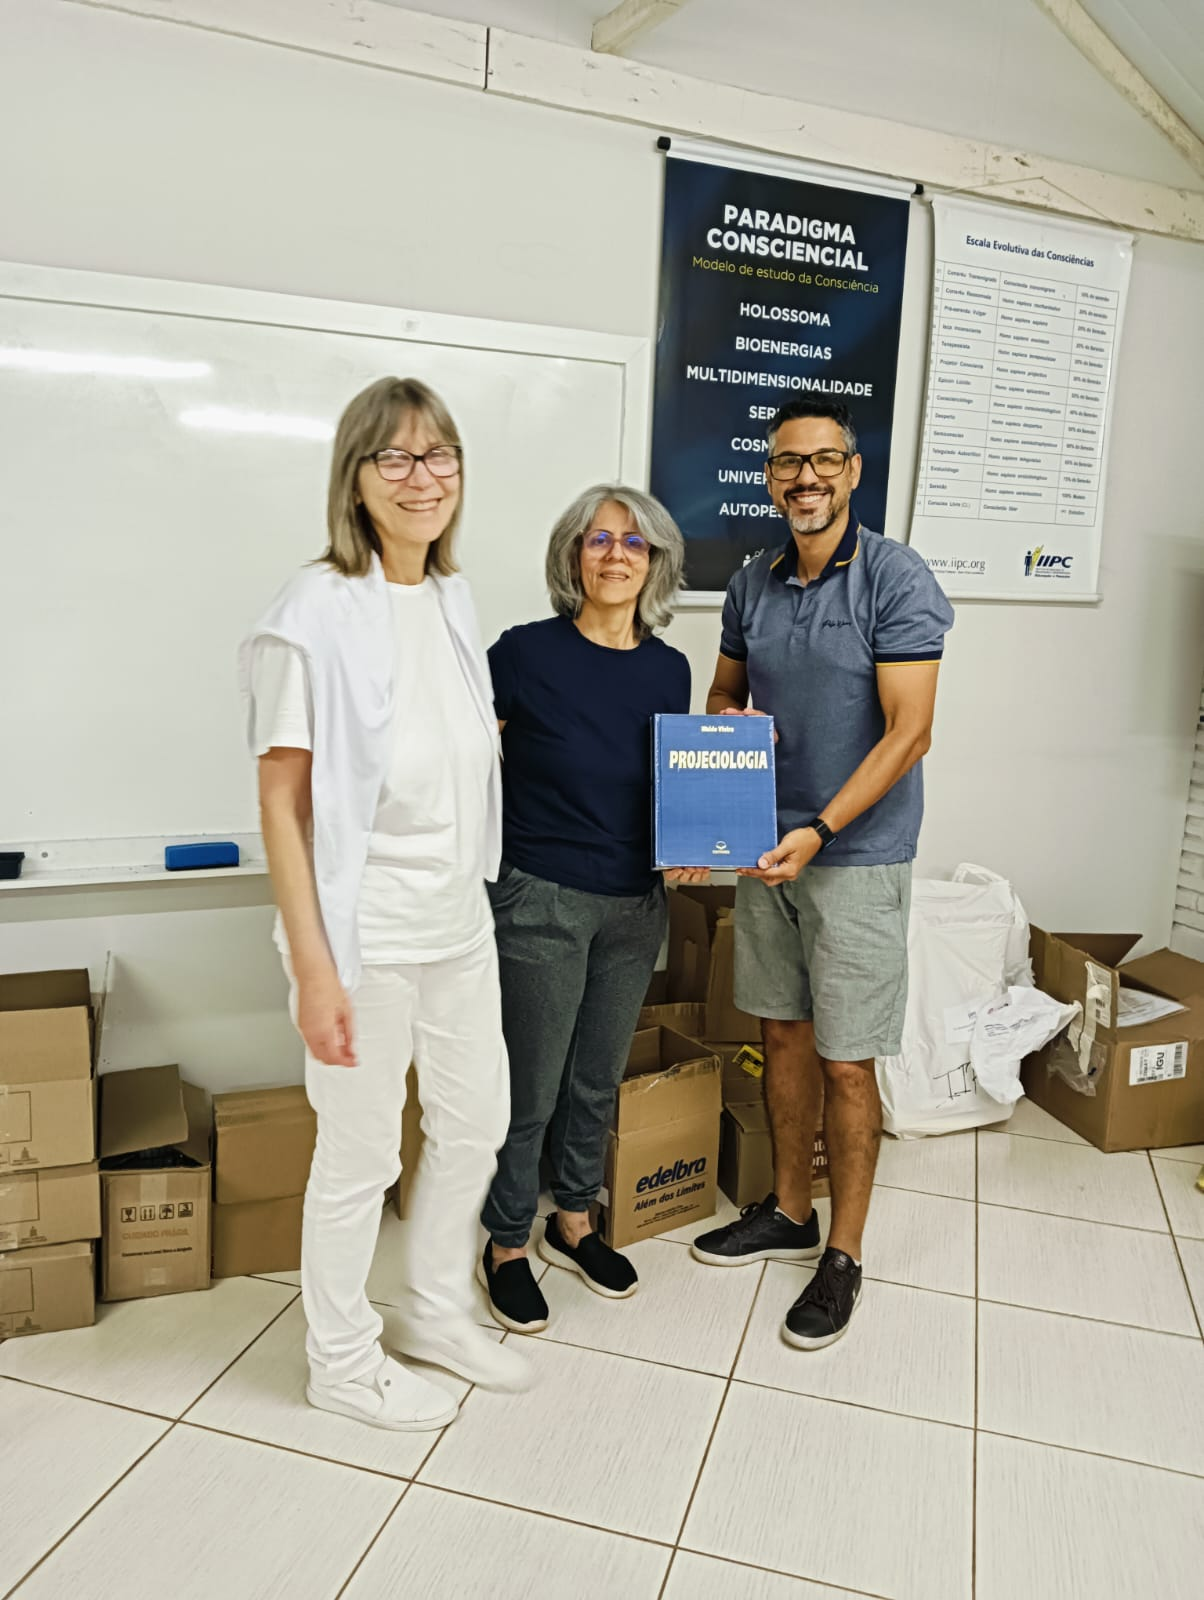
\includegraphics[height=8cm,trim={130 200 100 300},clip]{articles/parceria/imagens/editares-iipc.jpeg}
\end{center}


    
%    \begin{multicols}{2}


%\begin{wrapfigure}[11]{o}{0.5\textwidth}
%  %\begin{left}
%  %\vspace{-15mm}
%  %\hspace{1mm}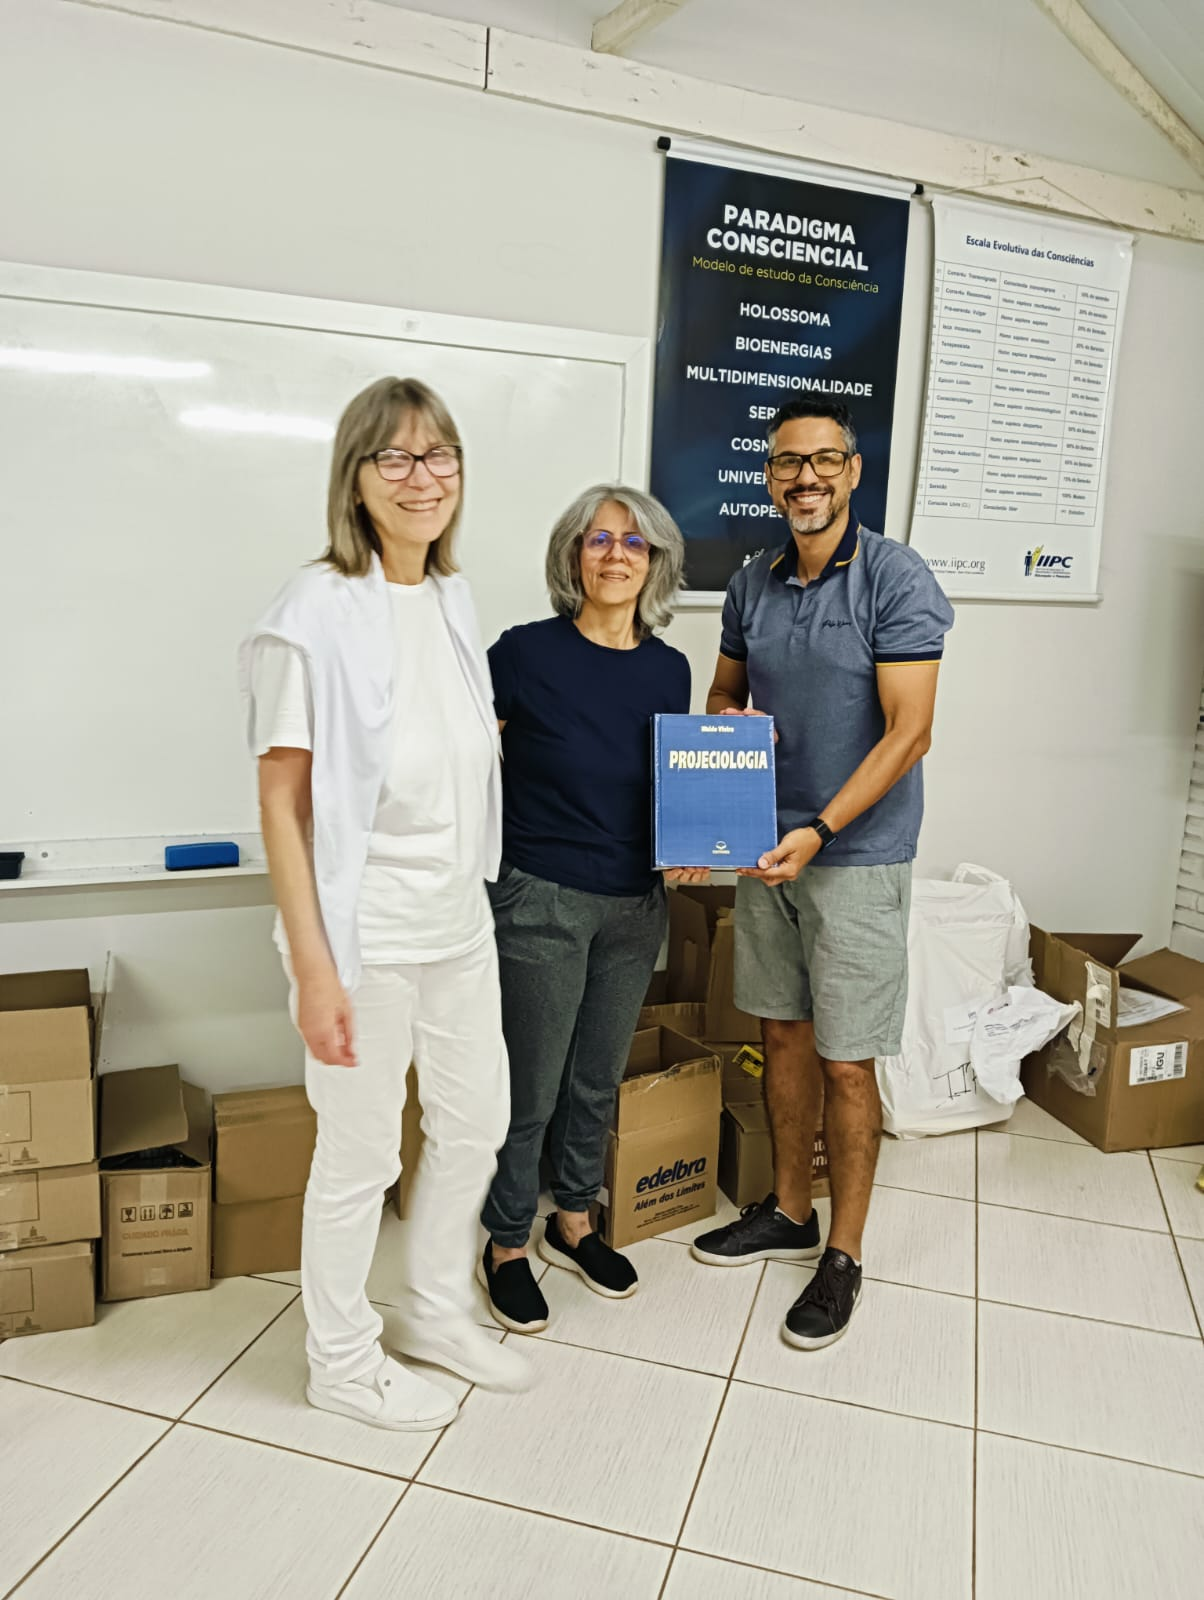
\includegraphics[height=10cm]{articles/parceria/imagens/editares-iipc.jpeg}
%  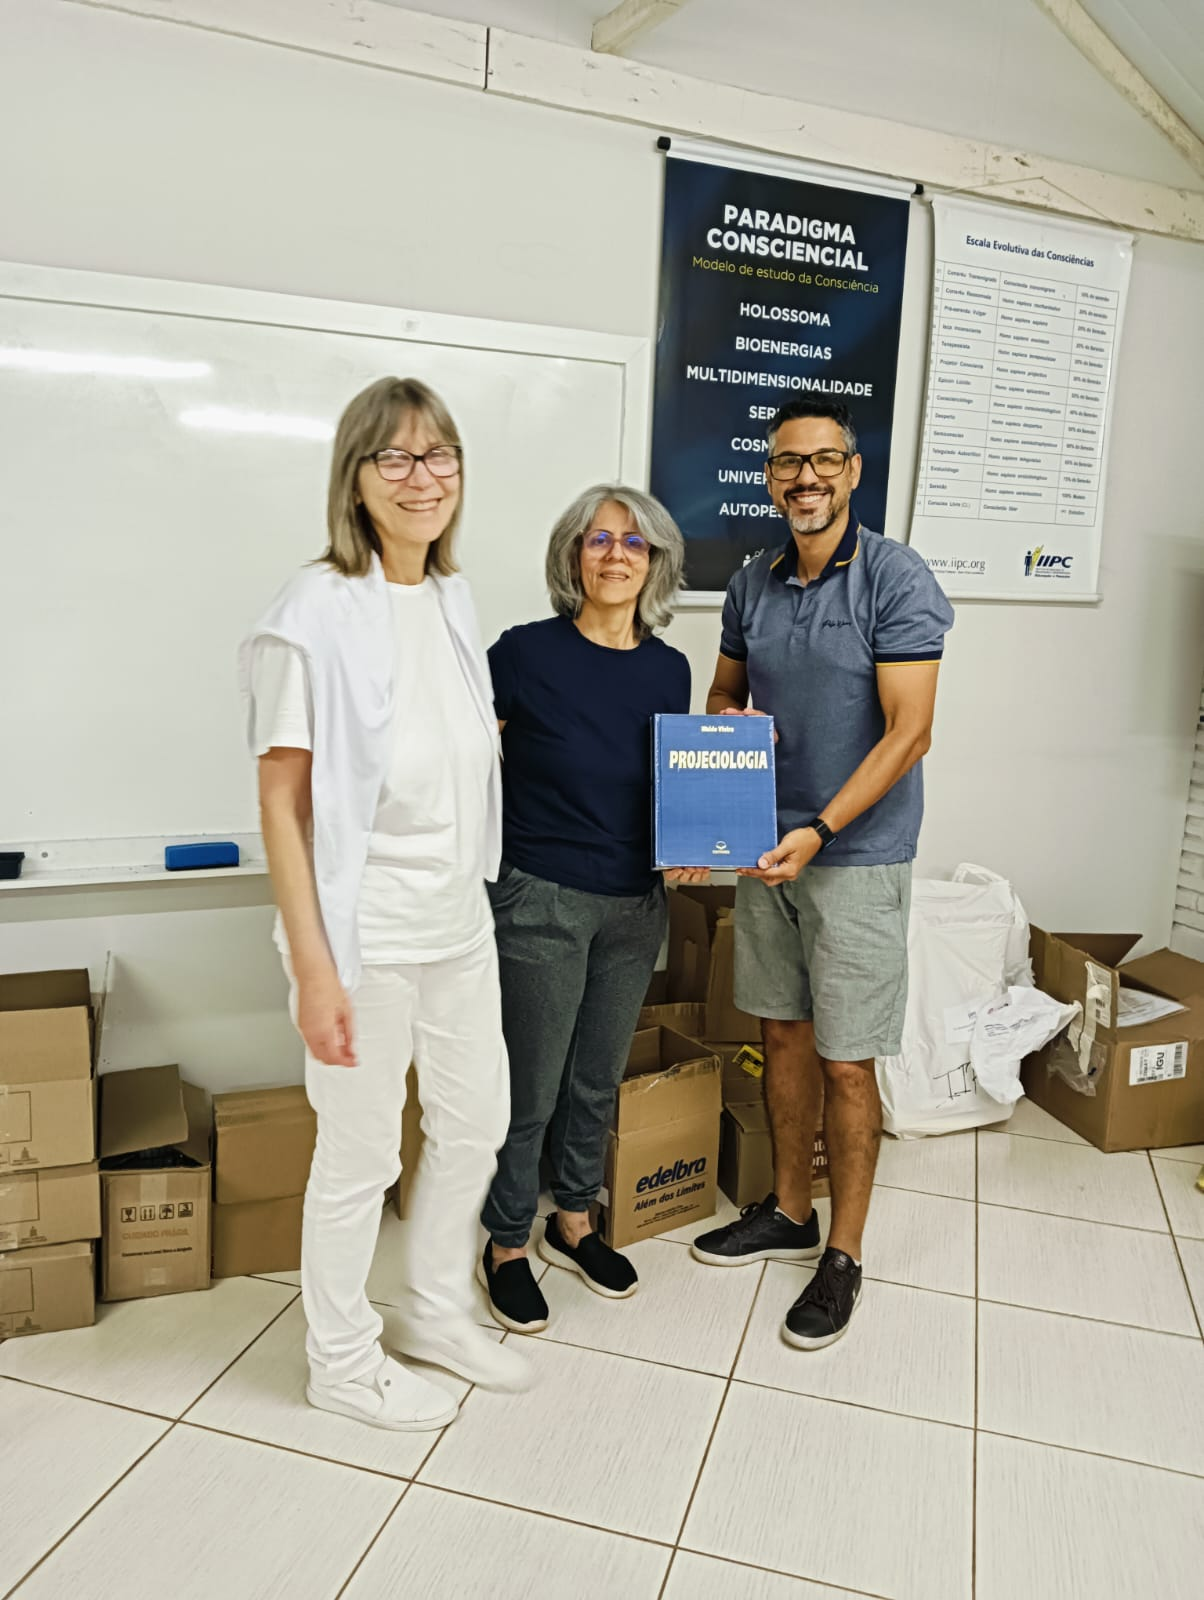
\includegraphics[height=8cm,trim={130 200 100 300},clip]{articles/parceria/imagens/editares-iipc.jpeg}
%  %\end{left}
%\end{wrapfigure}

\vspace{5mm}

Neste ano, a Editares, coordenada pelas voluntárias Ana Claudia Prado e Magda Stapf Amancio, celebra acordo exitoso com a coordenação geral e equipe do IIPC, representados pelos coordenadores gerais Gabriel Araújo e Ailton Maia, pelo qual \textbf{as obras conscienciológicas} estão sendo disponibilizadas para compra nos acervos dos \emph{Centros Educacionais de Autopesquisa} (CEAs) do \emph{Instituto Internacional de Projeciologia e Cons­cienciologia} (IIPC).

A renovação dessa parceria, além de possibilitar a melhoria logística da distri­buição comercial desses livros, auxiliará na ampliação da difusão tarística dos livros pu­blicados por autores conscienciológicos, ao permitir o acesso físico às gestações conscien­ciais para os visitantes e voluntários nos CEAs do IIPC.

\vspace{5mm}

\begin{center}
    
\includegraphics[height=4cm]{images/Logo-Editares-com-Marca-Registrada.png}
    \hspace{3cm}
    
\includegraphics[height=4cm]{images/IIPC_logo.png} 
\end{center}


% \begin{quote}
% \emph{Por: Ricardo Rezende}
% \emph{Voluntário do Setor Comercial da Editares}
% \emph{{[}FOTO DO AUTOR{]}}
% \end{quote}



%\emph{Editoras da Revista Editares}

%\emph{{[}Foto das autoras{]}}

%\emph{{[}INSERIR MOCKUP DA REVISTA QUE ESTÁ NA PASTA MATÉRIA 6{]}}


%\begin{center}
%    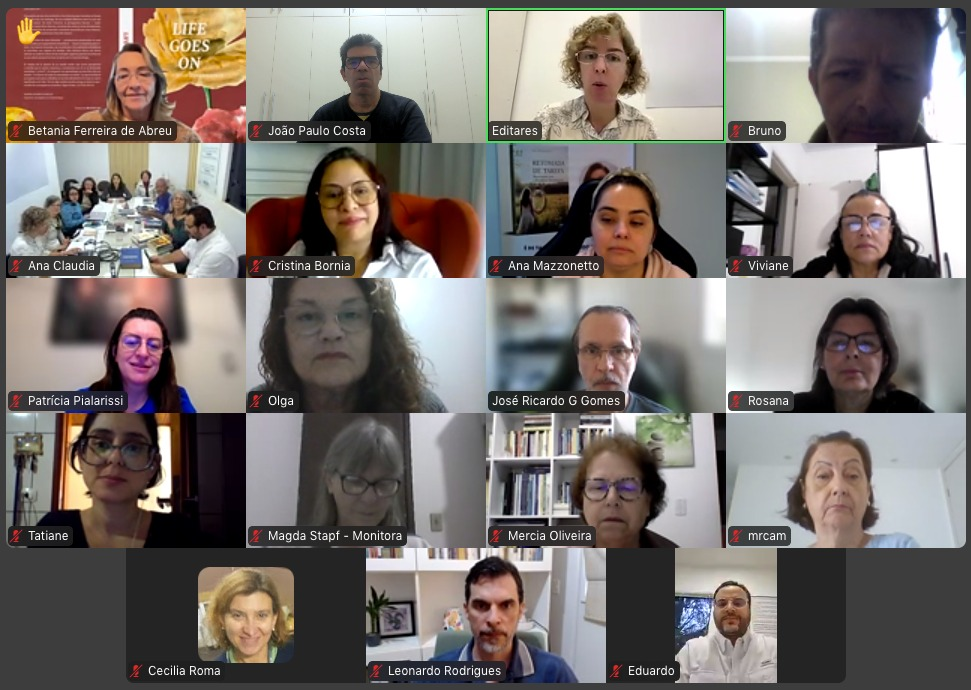
\includegraphics[width=9cm]{articles/atualizacoes/fotos/escola-editores/escola-editores1.jpeg} 
%\end{center}


%    \end{multicols}
\end{document}
